\documentclass[9pt]{beamer}
\mode<presentation>
\usepackage[T1]{fontenc}
\usepackage{color}
\usepackage{graphicx}
\usepackage{natbib}
\usepackage{tikz}
\usetikzlibrary{shapes.geometric}
\usepackage{xmpmulti}
\usepackage{animate}
\usepackage{tcolorbox}
\usepackage{amsmath}
\usepackage{gensymb}
\usepackage{csquotes}
\usepackage{bibentry}
\nobibliography*

%\usetheme{Singapore}
%\usecolortheme{seahorse}

\usefonttheme{professionalfonts}

\title[Word \& Doc Embeddings]{A Rapid Computer-assisted Systematic Map of Regional Climate Impacts}
%\author{Max Callaghan, Gerritt }
\institute[MCC]{
	
\includegraphics[height=1cm,width=2cm]{images/MCC_Logo_RZ_rgb.jpg}
}

\newif\ifframeinlbf
\frameinlbftrue
\makeatletter
\newcommand\listofframes{\@starttoc{lbf}}
\makeatother

\addtobeamertemplate{frametitle}{}{%
	\ifframeinlbf
	\addcontentsline{lbf}{section}{\protect\makebox[2em][l]{%
			\protect\usebeamercolor[fg]{structure}\insertframenumber\hfill}%
		\insertframetitle\par}%
	\else\fi
}

\newtheorem*{remark}{}

\bibliographystyle{apalike}

\begin{document}
	
\begin{frame}
	\titlepage
\end{frame}

\begin{frame}{Context}

Systematic assessments of the evidence on Climate Change like those conducted by the IPCC are vital.

\begin{columns}
	\begin{column}{0.618\linewidth}
		\begin{figure}
			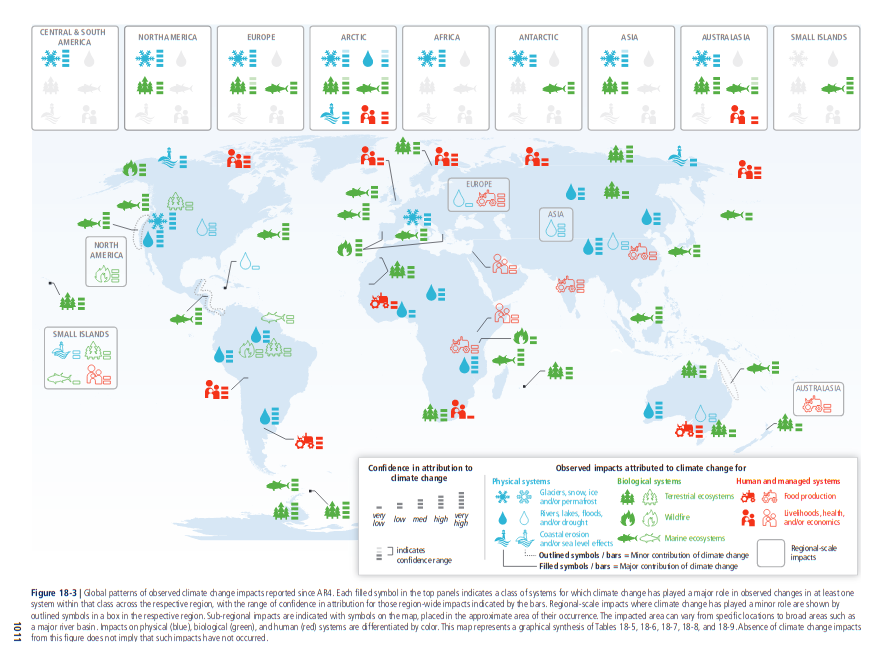
\includegraphics[width=\linewidth]{../map_18.png}<1->
		\end{figure}
	\end{column}
	\begin{column}{0.312\linewidth}

		\begin{figure}
			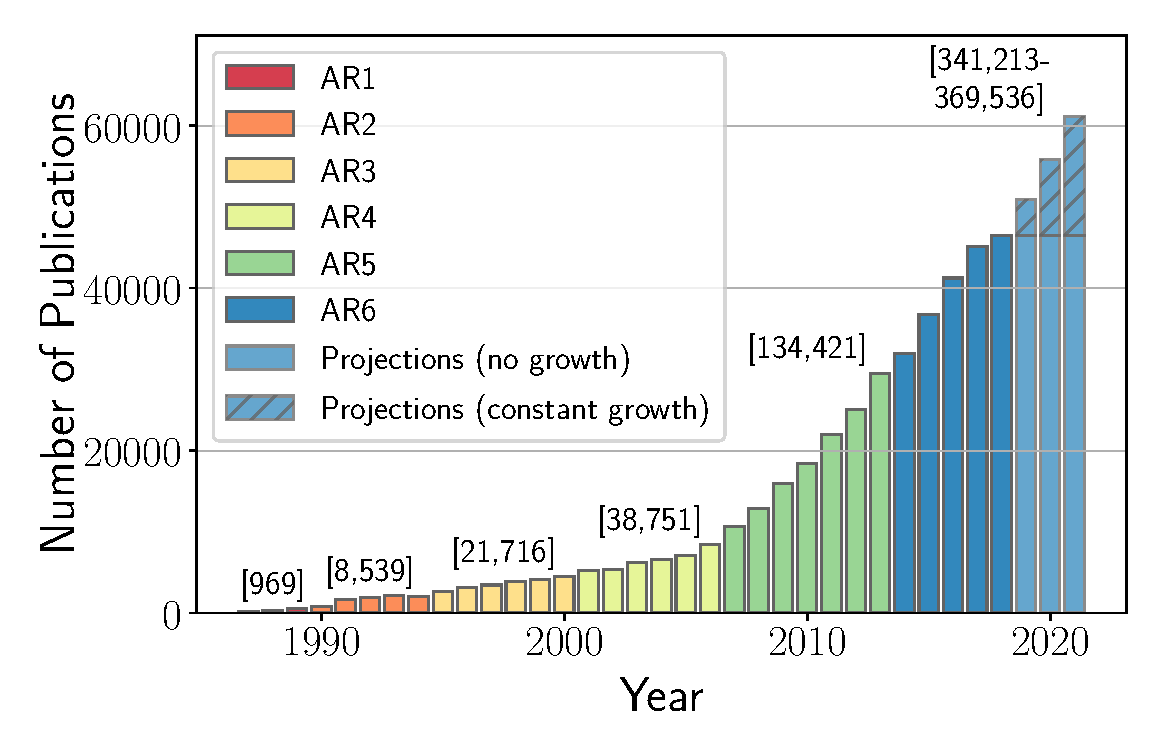
\includegraphics[width=\linewidth]{images/pubs_time_wgb_lp.pdf}<2->
		\end{figure}
	
		\begin{itemize}
			\small
			\item<2->These are challenged by big literature 
			\item<3->With more research out there, we need to be more systematic in assessing it
			\item<4->Machine learning can help
		\end{itemize}
	\end{column}
\end{columns}

\end{frame}


\begin{frame}{Rapid, Computer-assisted Systematic Mapping}



\begin{columns}
	\begin{column}{0.618\linewidth}
		\begin{figure}
			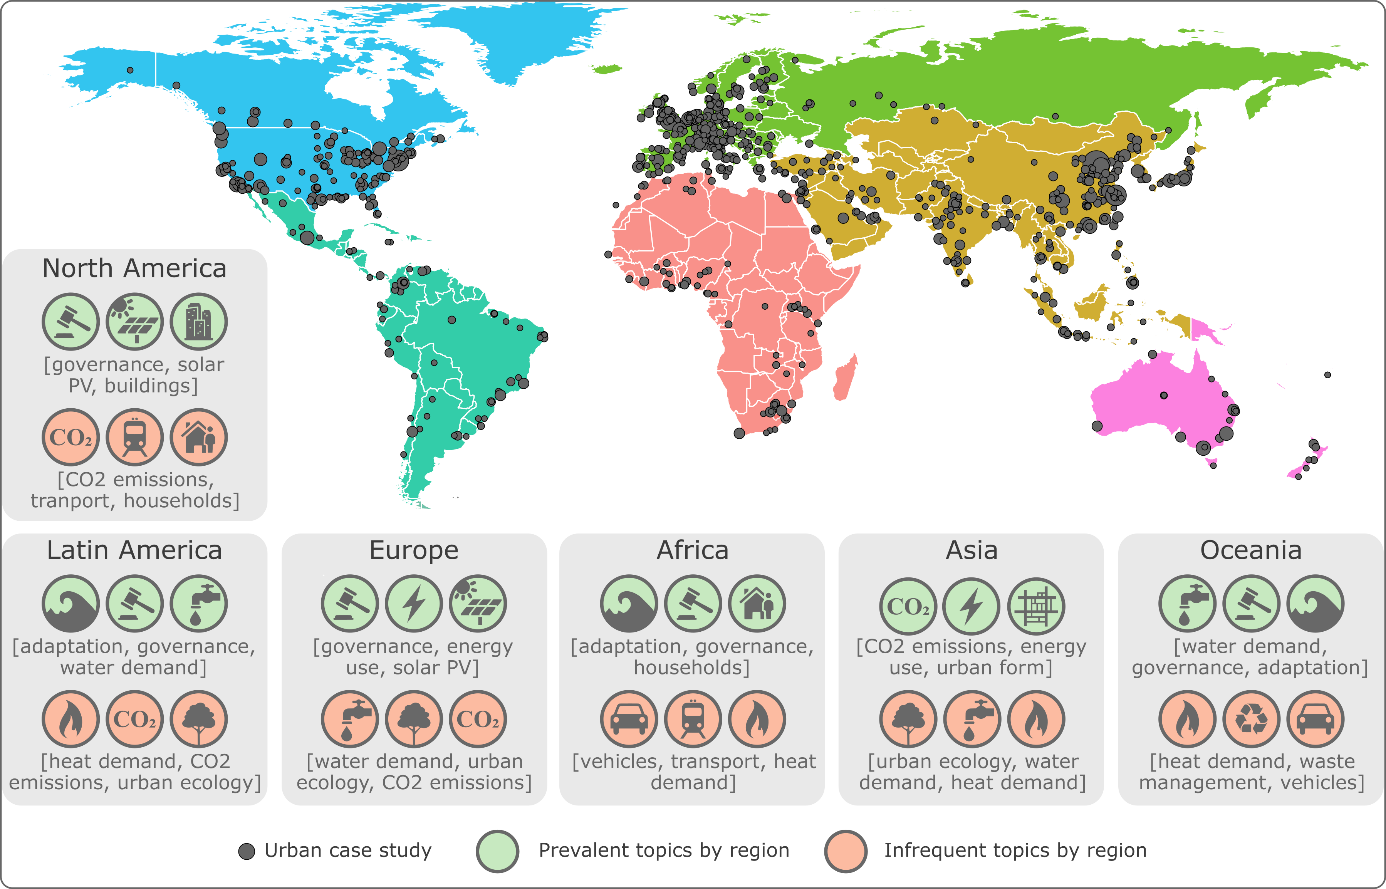
\includegraphics[width=\linewidth]{images/map.png}<1->
		
		\end{figure}
		\small\footnotesize\bibentry{Lamb2018d}
	\end{column}
	\begin{column}{0.312\linewidth}
		\begin{figure}
			%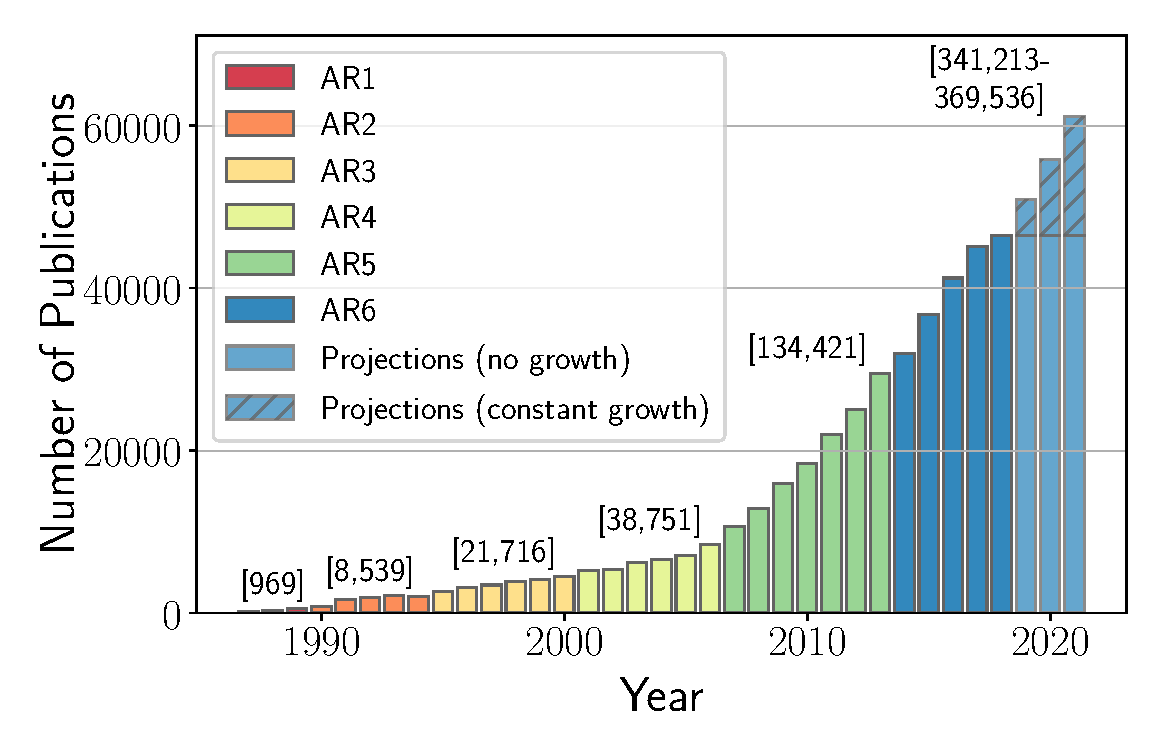
\includegraphics[width=\linewidth]{images/pubs_time_wgb_lp.pdf}<2->
		\end{figure}
	
	
		
		\begin{itemize}
			\small
			\item<1-> We produced a systematic map of the literature on urban mitigation
			\item<2-> Using topic models (unsupervised learning) we were able to describe the thematic content of research and show how that varied by region
		\end{itemize}
	\end{column}
\end{columns}

\only{\begin{tcolorbox}[colback=green!5,colframe=green!40!black]
	\noindent
	With regional impact attribution literature, we have specific categories we are looking for, and a small dataset of labelled documents 
\end{tcolorbox}}<3->


\end{frame}

\begin{frame}{Proposal}

We plan to use the labelled data from AR5 WGII Table 18-5 - 18-9 to train a classifier that can identify literature relevant to the different impact categories, in the corresponding map.

\bigskip

This will require more screening, for the generation of further validation and training data

\bigskip

The results can 

\begin{itemize}
	\item contribute to the production of the map in AR6
	\item inform us about research gaps
	\item enhance our understanding of the what literature what was included in the last map, and what, if any, other information could have been included
\end{itemize}



\end{frame}



\begin{frame}{AR5 Data}

	\begin{columns}
		\begin{column}{0.618\linewidth}
			\begin{figure}
				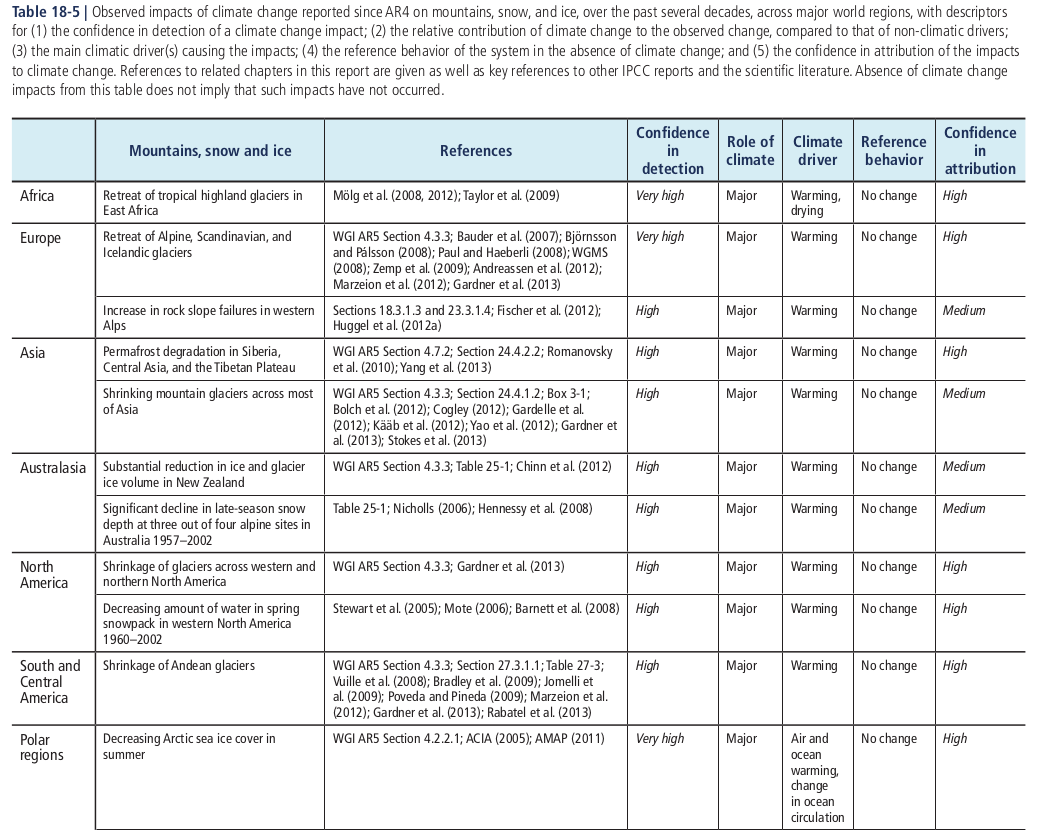
\includegraphics[width=\linewidth]{images/table.png}
			\end{figure}
		\end{column}
		\begin{column}{0.382\linewidth}
			257 Documents available in Web of Science from AR5 WGII Table 18-5 - 18-9
			
			\begin{figure}
				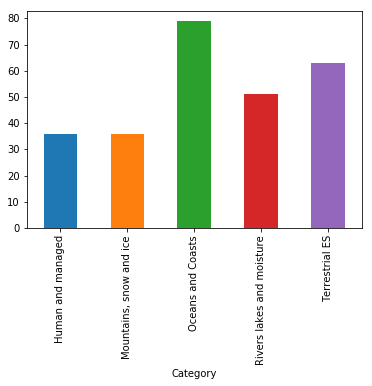
\includegraphics[width=\linewidth]{../plots/category_distribution.png}
			\end{figure}
		\end{column}
	\end{columns}



\end{frame}


\begin{frame}{Query Development}

The ideal query should contain \textit{all} documents included in the tables, along with \textit{all} additional relevant documents (untestable) and a hopefully minimal amount of irrelevant documents

\begin{figure}
	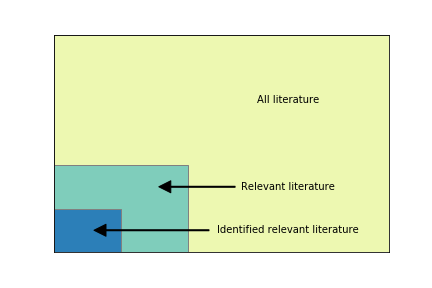
\includegraphics[width=0.7\linewidth]{../plots/basic_lit_plot.png}<1>
	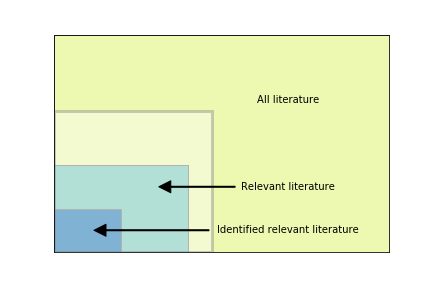
\includegraphics[width=0.7\linewidth]{../plots/lit_plot_query_1.png}<2>
	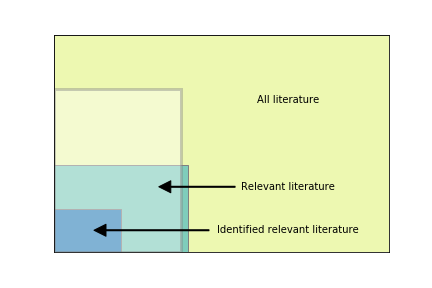
\includegraphics[width=0.7\linewidth]{../plots/lit_plot_query_3.png}<3>
	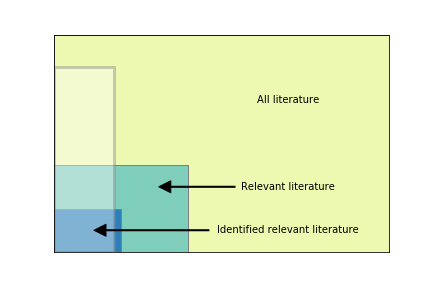
\includegraphics[width=0.7\linewidth]{../plots/lit_plot_query_2.png}<4>
\end{figure}

\end{frame}

\begin{frame}{Query Development}

I built a query that returns all identified documents by assembling keywords on three themes

\medskip

\begin{columns}[t]
	\begin{column}{0.33\linewidth}
		\textbf{Climate}
		
		\scriptsize
		
		TS=("climate model" OR "elevated* temperatur" OR "ocean* warming" OR "saline* intrusion" OR "chang* climat" OR "environment* change" OR "climat* change" OR "climat* warm" OR "warming* climat" OR "climat* varia" OR "global* warming" OR "global* change" OR "greenhouse* effect" OR "anthropogen*" OR "sea* level" OR "precipitation variabil*" OR "precipitation change*" OR "temperature* impact" OR "environmental* variab" OR "weather* pattern" OR "weather* factor*" OR "climat*") OR TS=("change* NEAR/5  cryosphere" OR "increase* NEAR/3  temperatur*")
	\end{column}
	\begin{column}{0.33\linewidth}
		\textbf{Impacts}
		
		\scriptsize
		TS=("impact*" OR "specie*" OR "mortality*" OR "ecosystem*" OR "mass balance" OR "flood*" OR "drought" OR "disease*" OR "adaptation" OR "malaria" OR "fire" OR "water scarcity" OR "water supply" OR "permafrost" OR "biological response" OR "food availability" OR "food security" OR "vegetation dynamic*" OR "cyclone*" OR "yield*" OR "snow water equival*" OR "surface temp*") OR TS=("glacier* NEAR/3  melt*" OR "glacier* NEAR/3  mass*" OR "erosion* NEAR/5  coast*" OR "glacier* NEAR/5  retreat*" OR "rainfall* NEAR/5  reduc*" OR "coral* NEAR/5  stress*" OR "precip* NEAR/5  *crease*" OR "river NEAR/5  flow")
	\end{column}
	\begin{column}{0.33\linewidth}
		\textbf{Attribution}
		
		\scriptsize
		TS=("recent" OR "current" OR "modern" OR "observ*" OR "evidence*" OR "past" OR "local" OR "region*" OR "significant" OR "driver*" OR "response" OR "were responsible" OR "was responsible" OR "exhibited" OR "witnessed" OR "attribut*" OR "has increased" OR "has decreased" OR "histor*" OR "correlation" OR "evaluation")
	\end{column}
\end{columns}

\medskip



\end{frame}

\begin{frame}{Machine Learning Approach}

\begin{itemize}
	\item We use the text of the documents to train a model to categorise the documents we know the categories for
	\item We use that model to predict the categories of documents we haven't seen yet
	\item We screen these documents, providing validation and more training data
\end{itemize}

\end{frame}

\begin{frame}{Proof of Concept}

\begin{figure}
	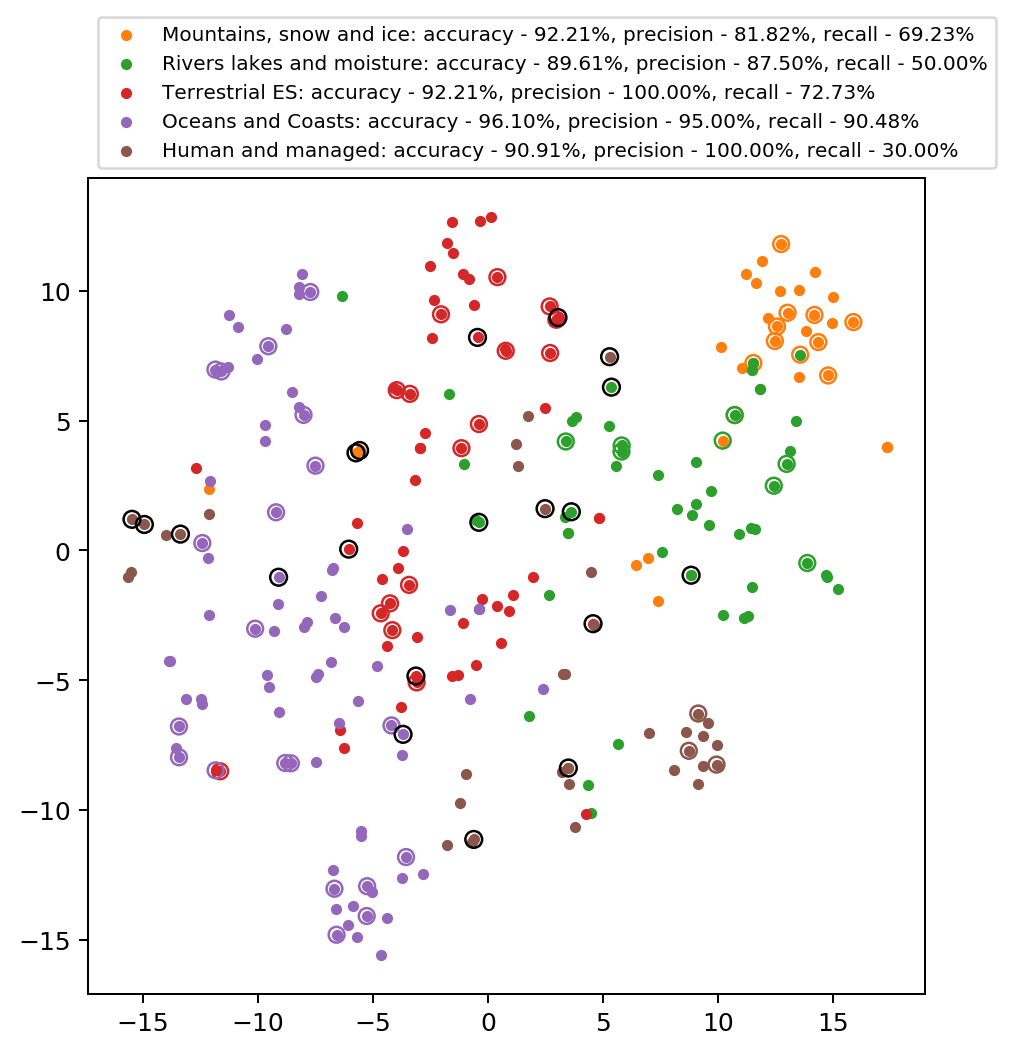
\includegraphics[width=0.75\linewidth]{../plots/original_predictions.png}
\end{figure}

\end{frame}

\begin{frame}{Proof of Concept}

\begin{figure}
	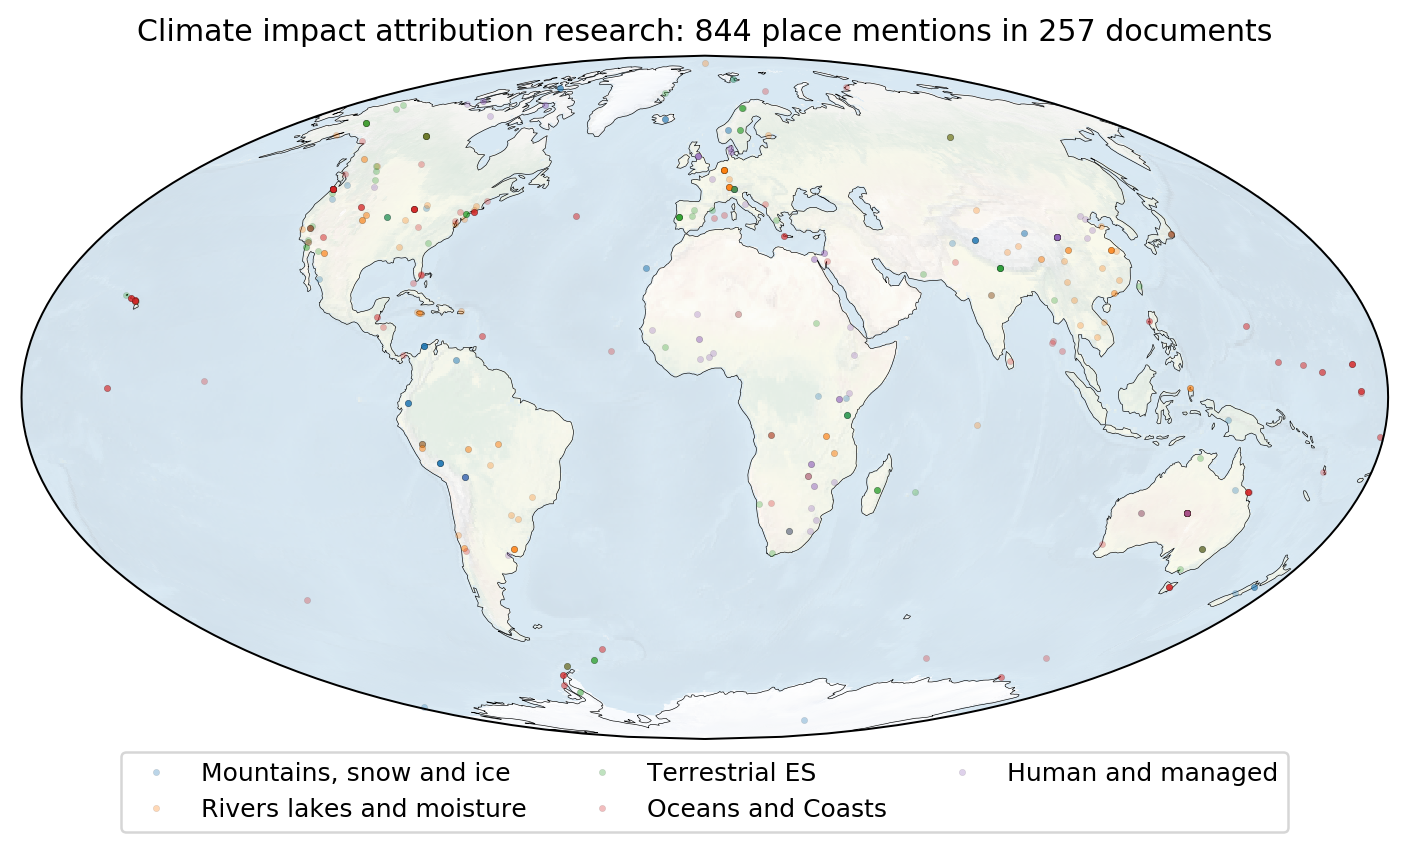
\includegraphics[width=\linewidth]{../plots/original_map.png}
\end{figure}

\end{frame}

\begin{frame}{Proof of Concept - unseen data}

	We view the same documents in the context of a sample of 10,000 new documents

	\begin{columns}
	\begin{column}{0.618\linewidth}
		\begin{figure}
			%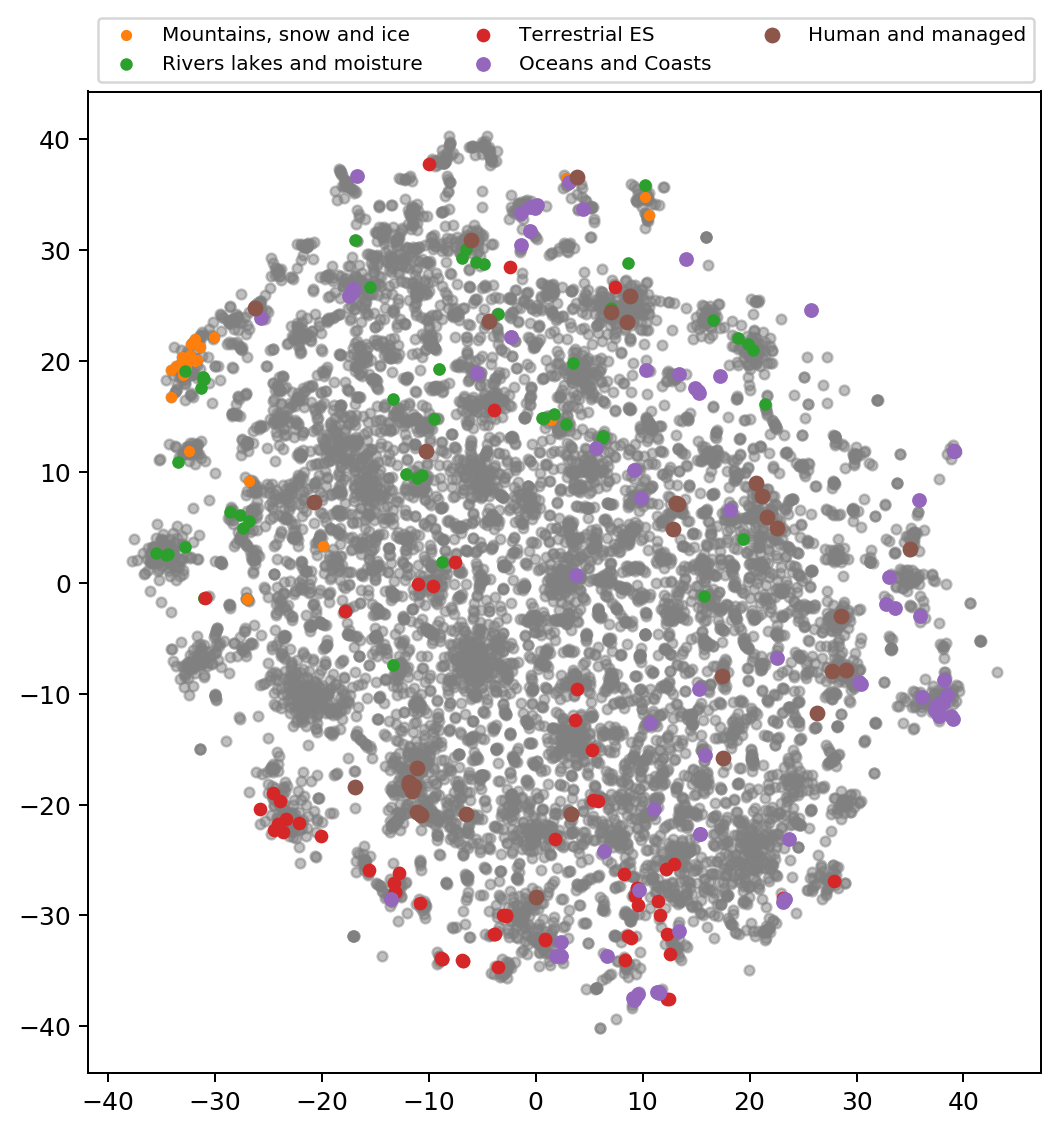
\includegraphics[width=\linewidth]{../plots/unseen_cats.png}<1>
			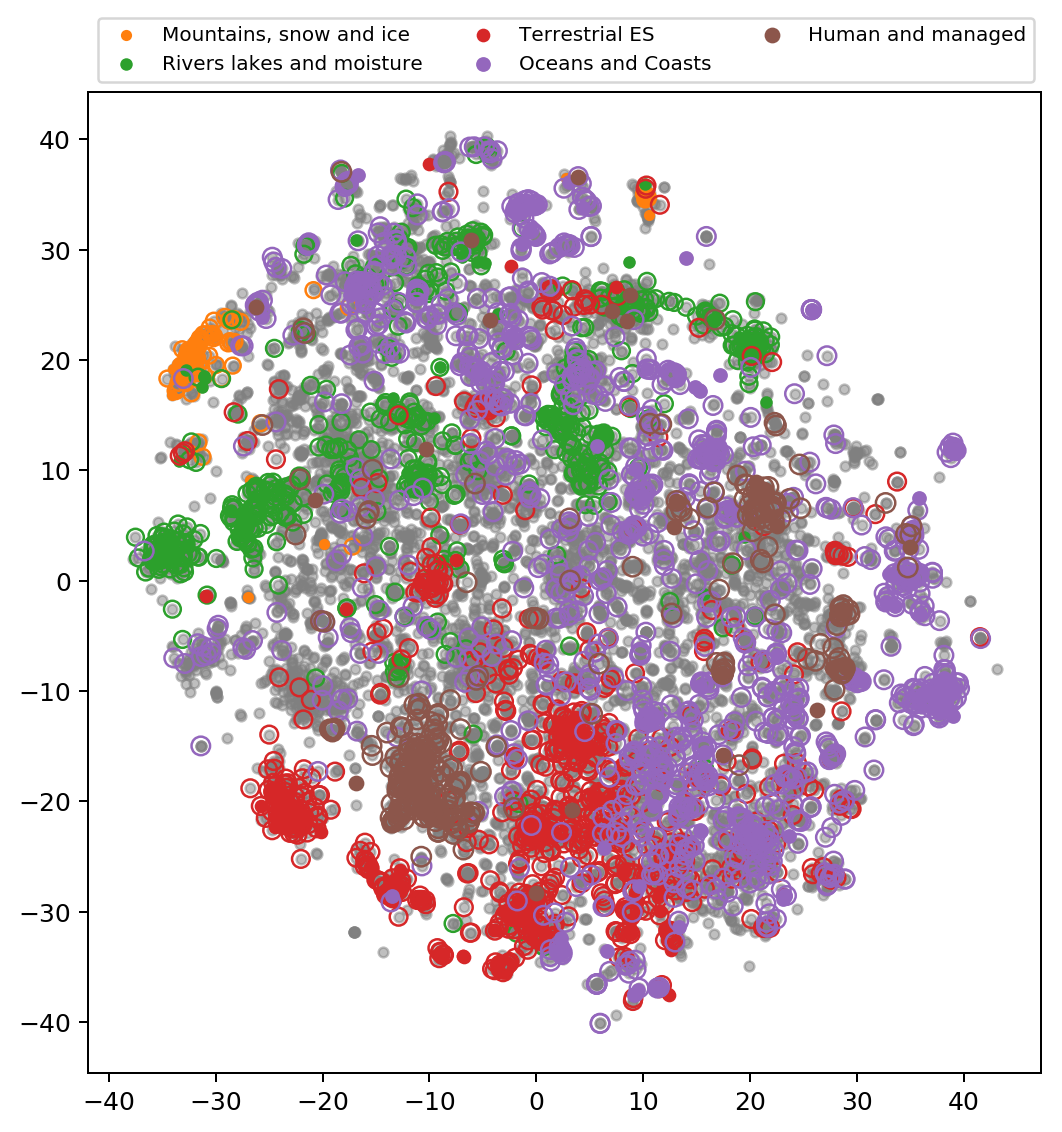
\includegraphics[width=\linewidth]{../plots/predicted_unseen_cats.png}<2->
		\end{figure}
	\end{column}
	\begin{column}{0.382\linewidth}
		\begin{itemize}
			\item<2-> We can train the model on the known documents, and use it to predict the categories of the unseen documents
			\item<3-> About 40\% of documents are predicted to be relevant (!), but the model is only trained on positive cases
			
		\end{itemize}
		
		\begin{figure}
			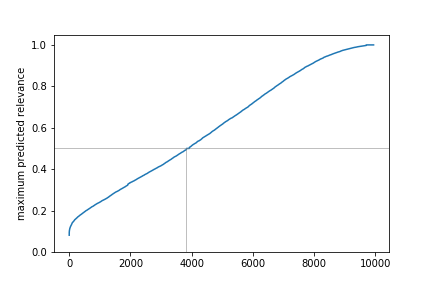
\includegraphics[width=\linewidth]{../plots/maximum_predicted_relevance.png}<3->
		\end{figure}
	\end{column}
\end{columns}

\end{frame}

\begin{frame}{Proof of Concept - unseen data}

\only{Recall the orignal map of places mentioned in the AR5 documents}<1>
\only{In just a sample of 10,000 documents, we have a lot more places mentioned, and regional concentrations are clearer}<2>

\begin{figure}
	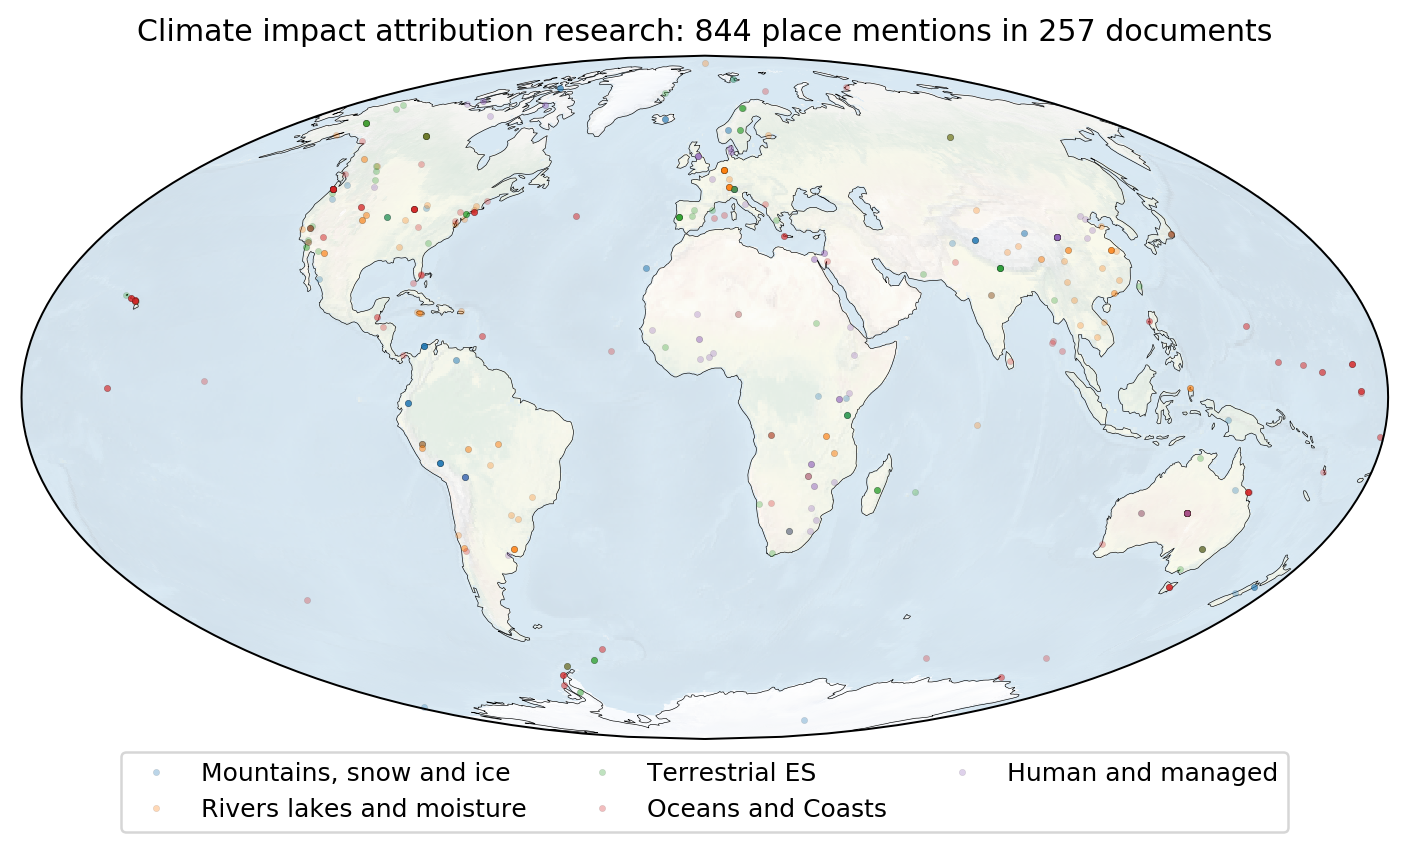
\includegraphics[width=\linewidth]{../plots/original_map.png}<1>
	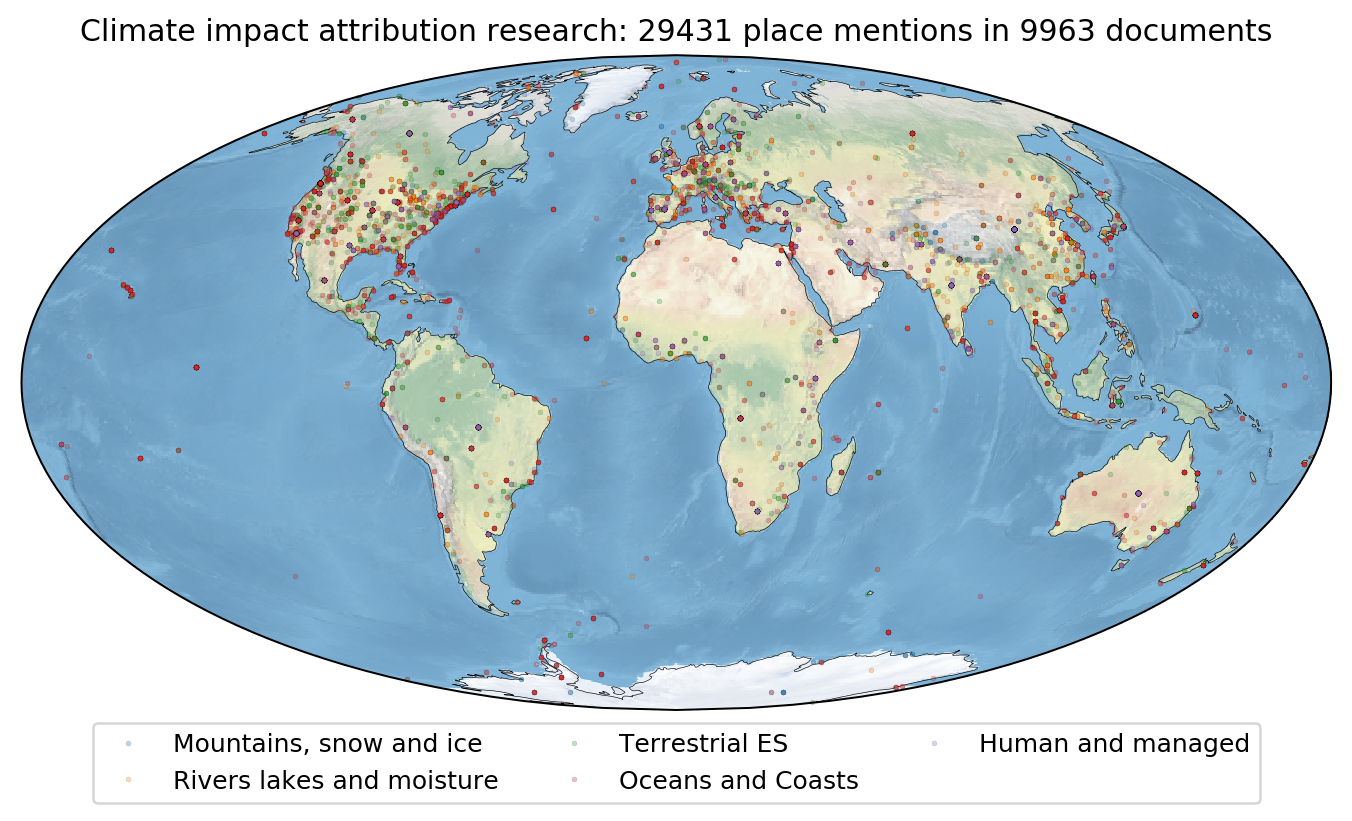
\includegraphics[width=\linewidth]{../plots/predicted_map.png}<2>
\end{figure}

\end{frame}

\begin{frame}{Screening so far}

\begin{itemize}
	\item A random sample of 500 documents
	\item A sample of 200 predicted to be relevant
	
\end{itemize}

\begin{figure}
	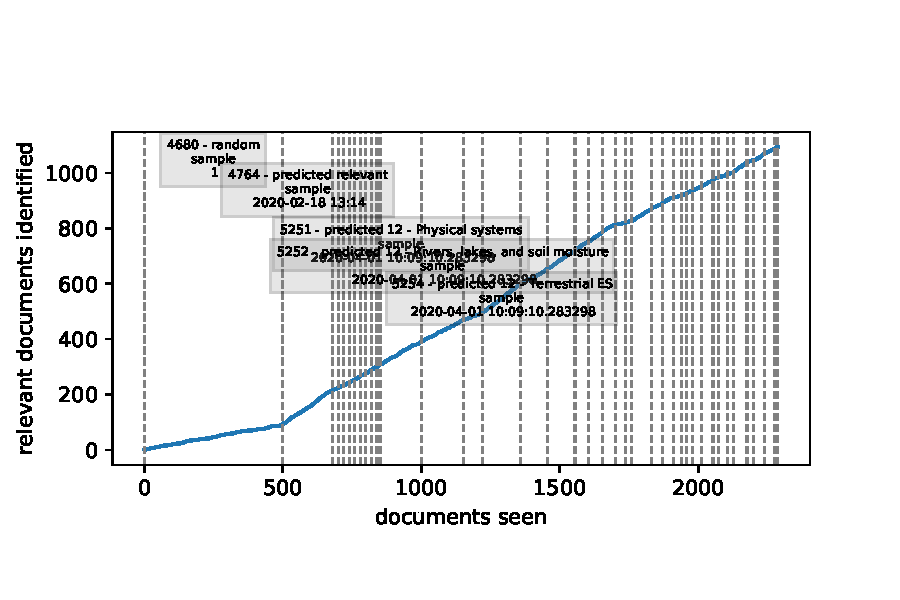
\includegraphics[width=\linewidth]{../plots/progress/reldocs_docs.pdf}
\end{figure}

\end{frame}

\begin{frame}{Screening task}

\only<1>{
\begin{figure}
	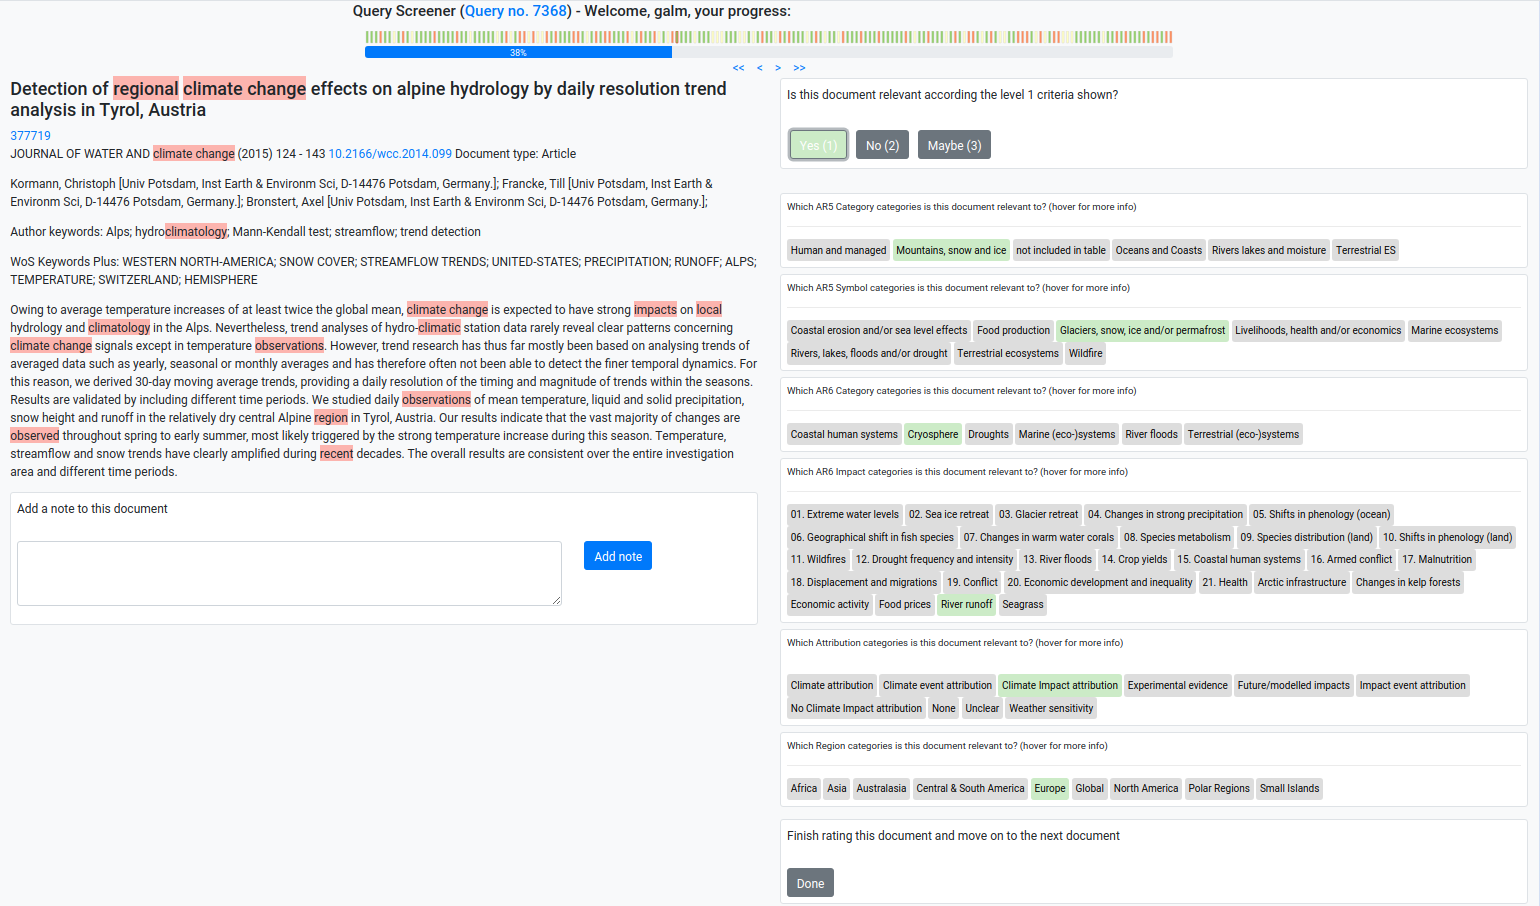
\includegraphics[width=\linewidth]{../literature_identification/screening_example/screen.png}
\end{figure}
}
\only<2>{
	\begin{figure}
		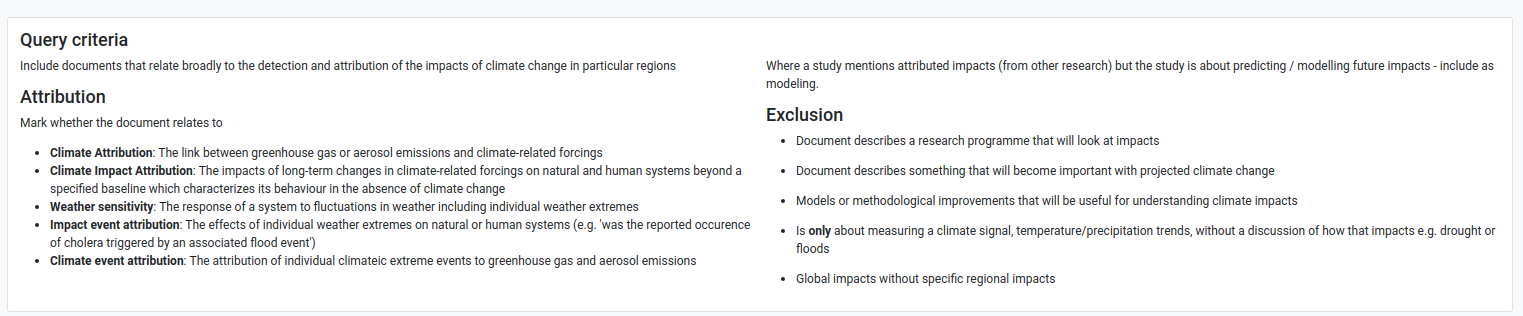
\includegraphics[width=\linewidth]{../literature_identification/screening_example/criteria.png}
	\end{figure}
}

\end{frame}

\begin{frame}{Screening task}

\begin{figure}
	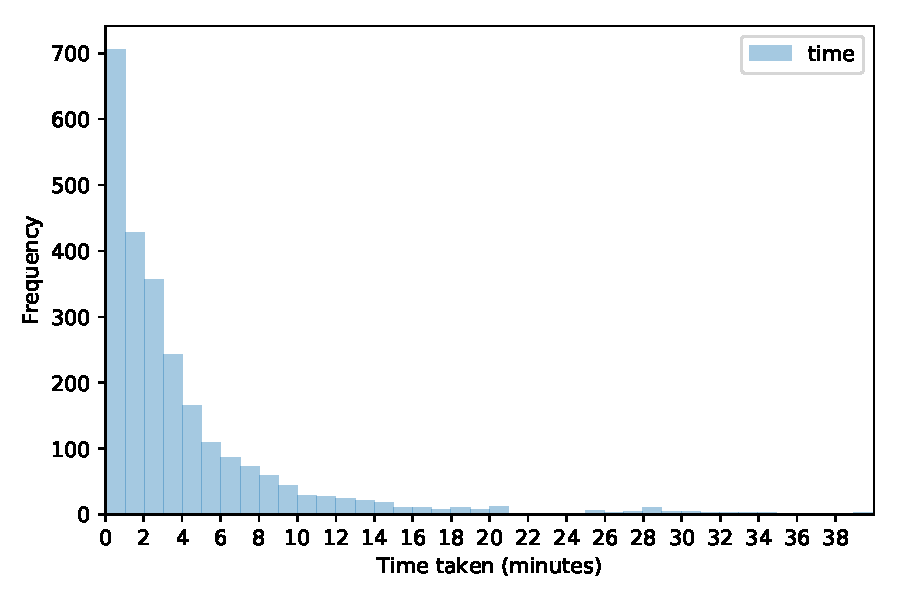
\includegraphics[width=\linewidth]{../plots/progress/time_taken_hist.pdf}
\end{figure}

\end{frame}

%%

\begin{frame}{Categories}

\only<1>{
\begin{figure}
	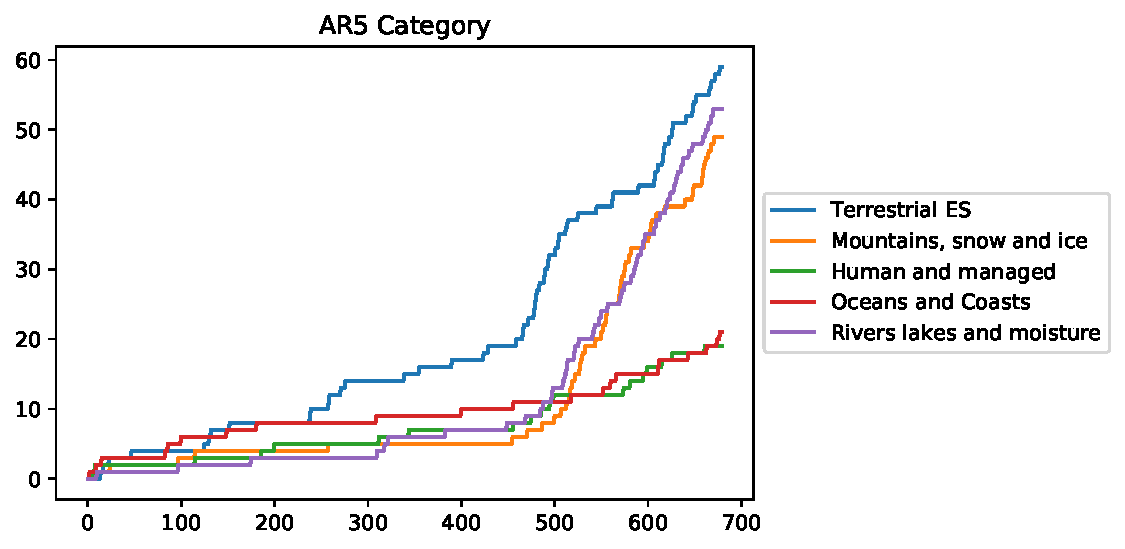
\includegraphics[width=\linewidth]{../plots/progress/AR5_Category.pdf}
\end{figure}
}

\only<2>{
\begin{figure}
	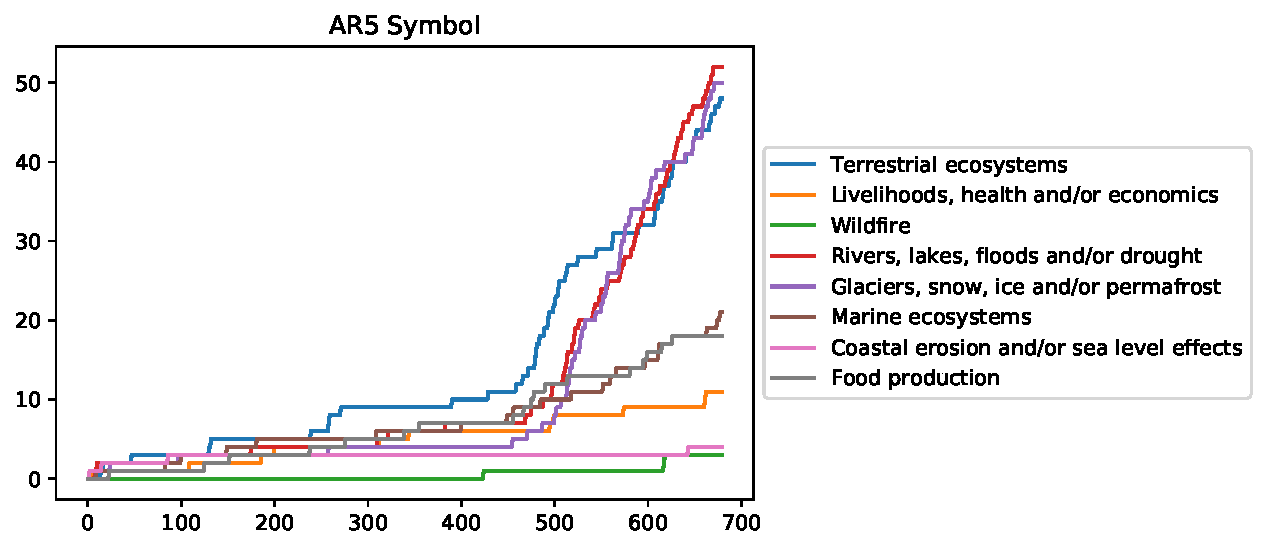
\includegraphics[width=\linewidth]{../plots/progress/AR5_Symbol.pdf}
\end{figure}
}

\only<3>{
	\begin{figure}
		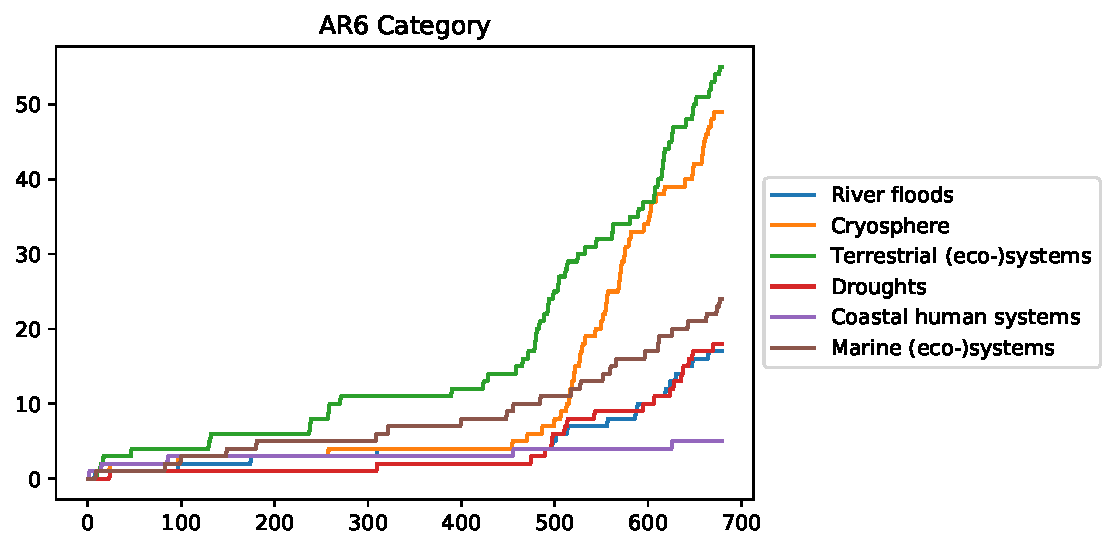
\includegraphics[width=\linewidth]{../plots/progress/AR6_Category.pdf}
	\end{figure}
}

\only<4>{
	\begin{figure}
		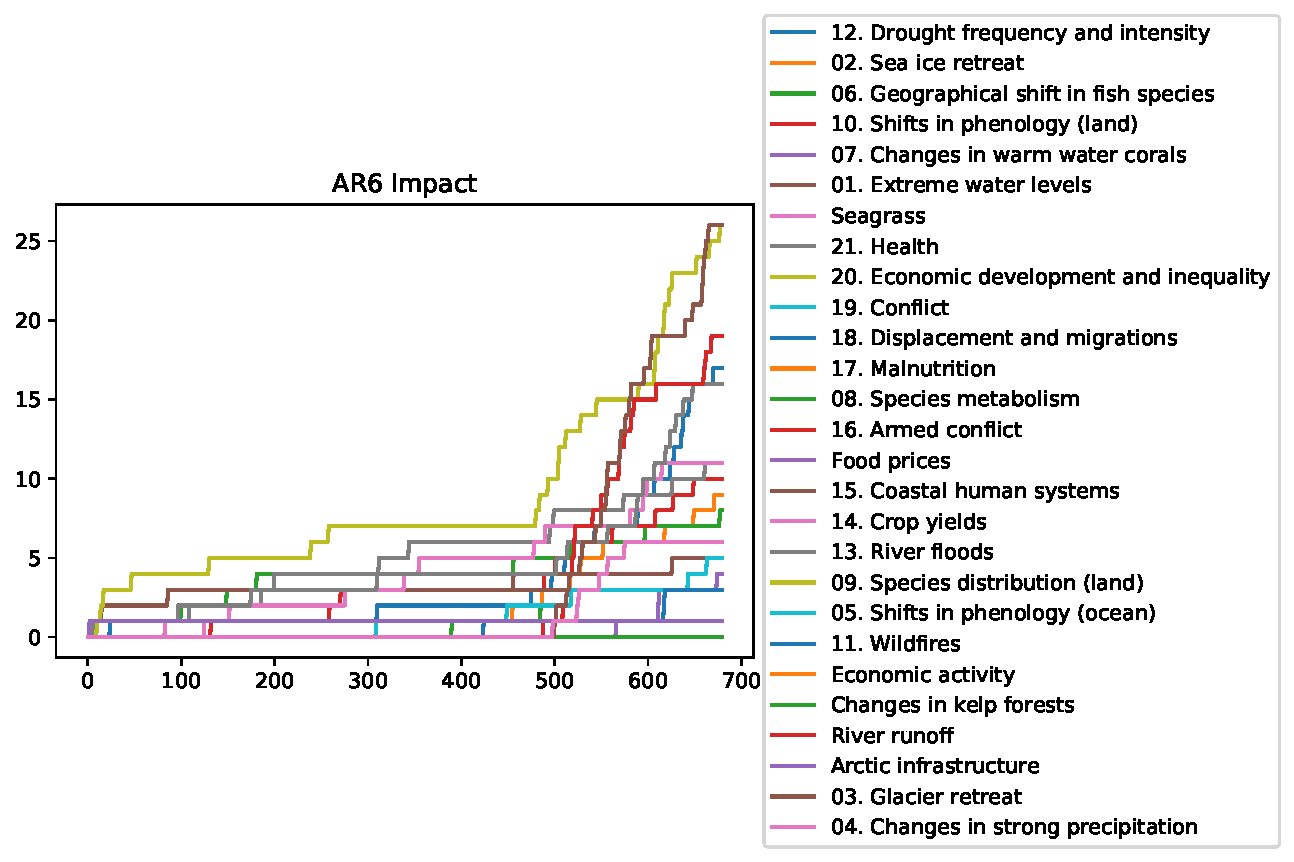
\includegraphics[width=\linewidth]{../plots/progress/AR6_Impact.pdf}
	\end{figure}
}

\only<5>{
	\begin{figure}
		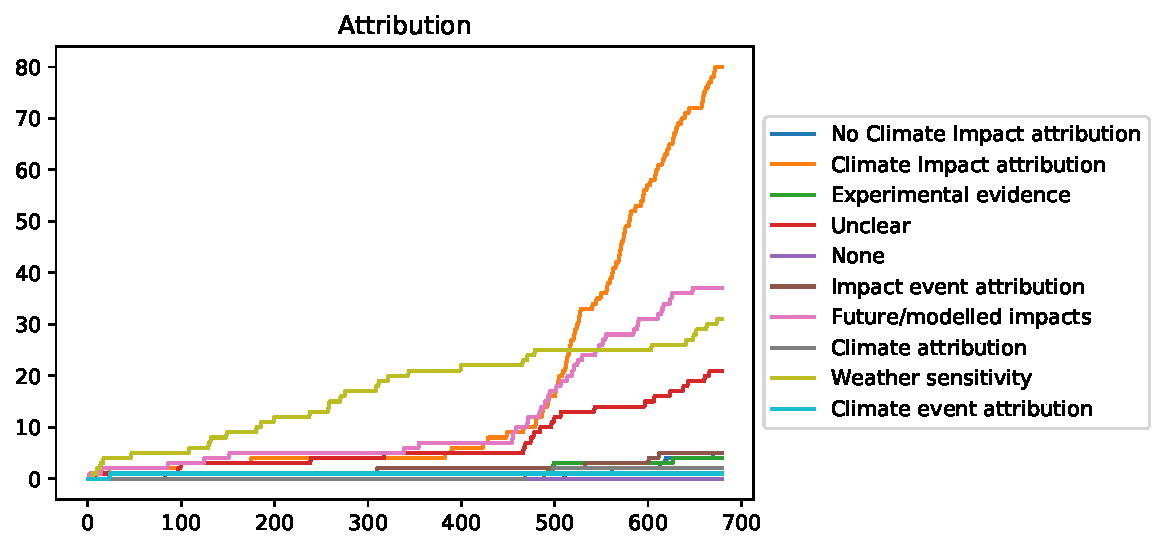
\includegraphics[width=\linewidth]{../plots/progress/Attribution.pdf}
	\end{figure}
}

\only<6>{
	\begin{figure}
		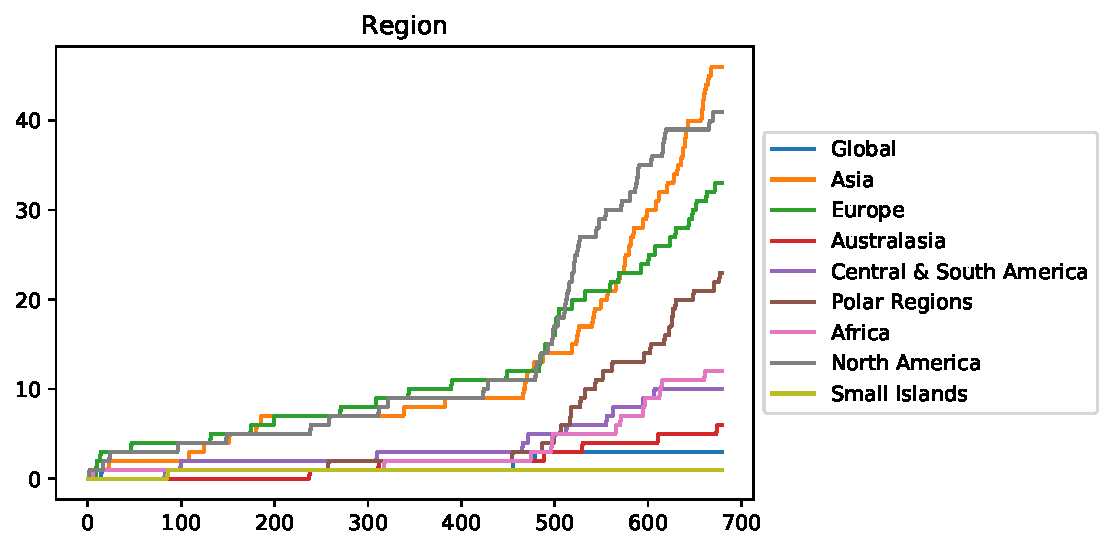
\includegraphics[width=\linewidth]{../plots/progress/Region.pdf}
	\end{figure}
}


\end{frame}

\begin{frame}{Category Overlap}

\begin{figure}	
	\hspace*{-0.05\linewidth}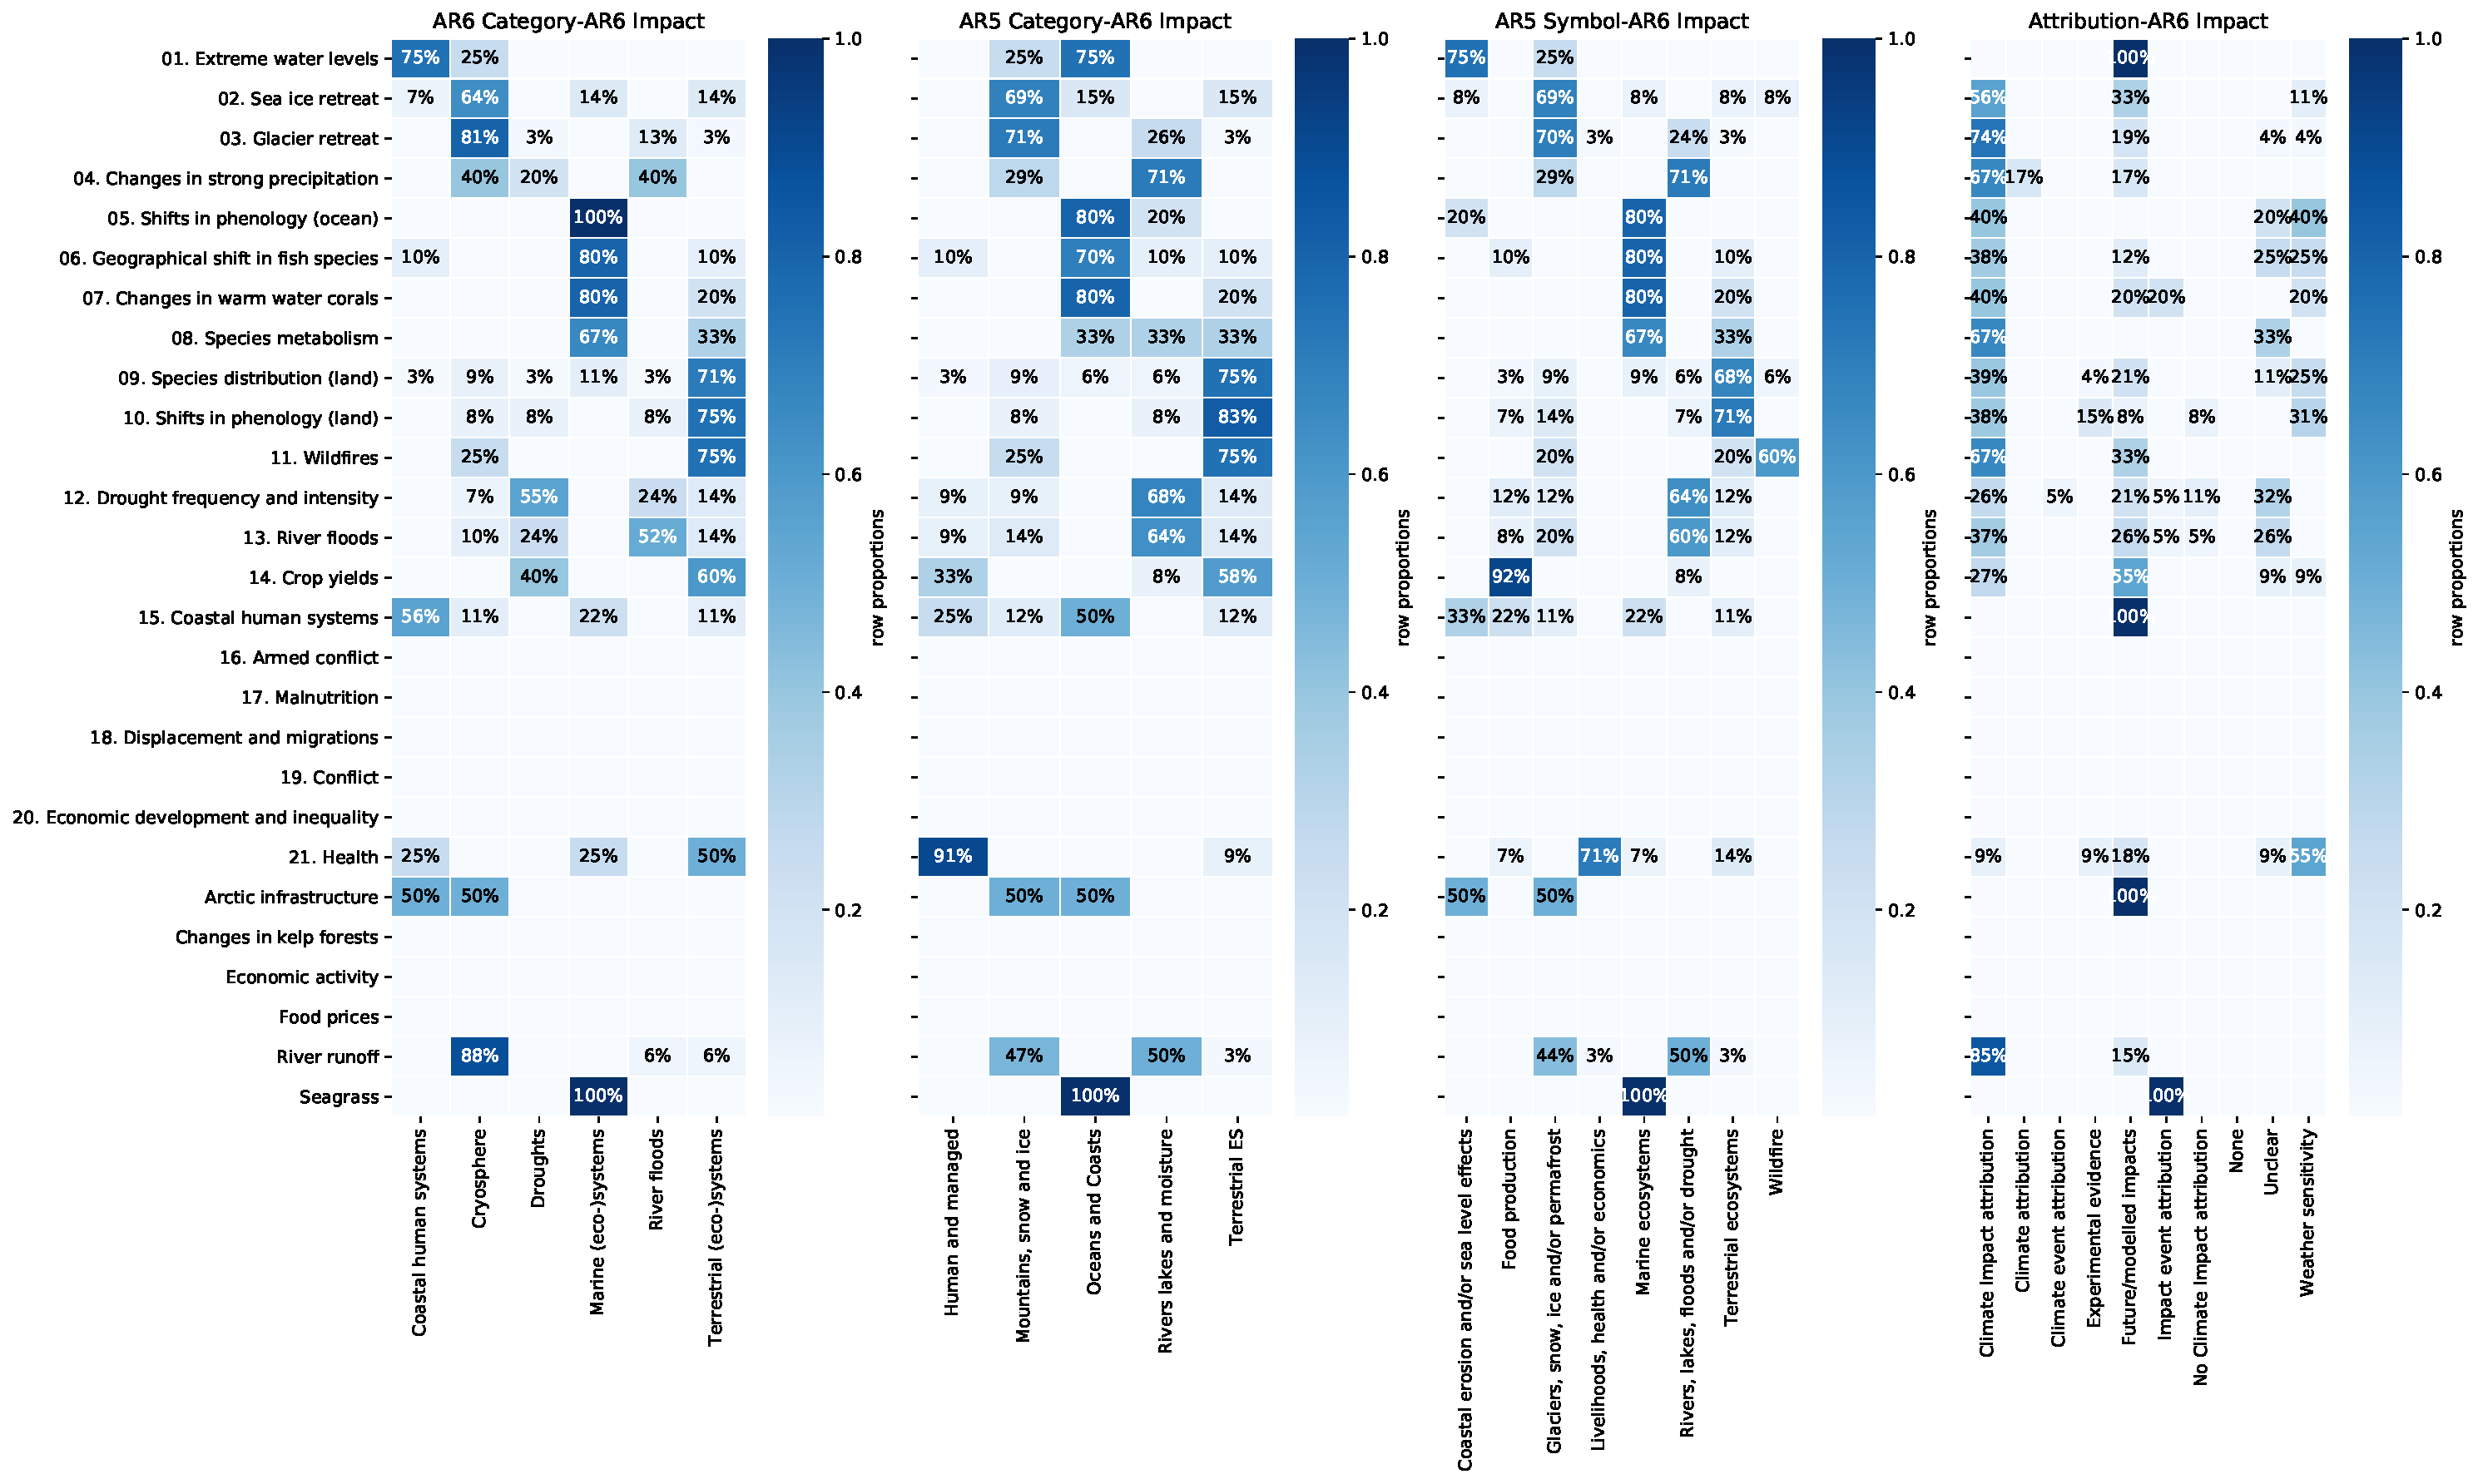
\includegraphics[width=1.1\linewidth]{../plots/progress/AR6_Impact_overlap.pdf}
\end{figure}

\end{frame}

\begin{frame}{Learning}

\begin{figure}	
	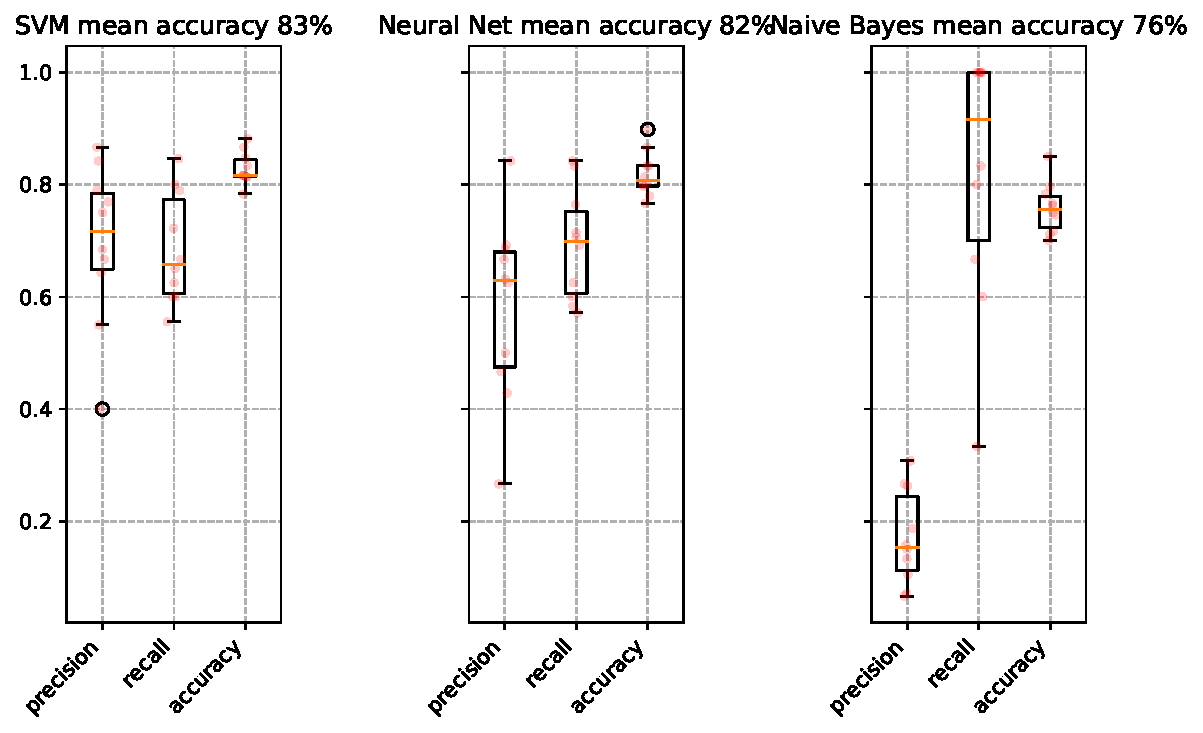
\includegraphics[width=1\linewidth]{../plots/prediction_models/relevance_prediction_2020-03-12_11:36:25.pdf}
\end{figure}

\end{frame}

\begin{frame}{Next steps}

\begin{columns}[t]
	\begin{column}{0.5\linewidth}
		\textbf{Coding}
		\begin{itemize}
			\item Adjusting criteria
			\item Adjusting categories
			\item Other information to extract
			\item Distribution of categories to team
			\item Testing
			\item Hackathon(s) [late March - end of April]
		\end{itemize}
	\end{column}
	\begin{column}{0.5\linewidth}
		\textbf{In parallel}
		\begin{itemize}
			\item Paper outline
			\item Maps
			\item Analysis
			\item Draft paper
		\end{itemize}
	\end{column}
\end{columns}

\medskip

\hrule

\medskip

Submission by 1 July 2020

\end{frame}



\begin{frame}{References}
\bibliography{../mendeley}
\end{frame}


\end{document}